\documentclass[a4paper,11pt]{article}
\usepackage[margin=2cm]{geometry}
\usepackage{graphicx}
\usepackage{amsmath}
\begin{document}
\section*{Results: damage\_front}
\begin{figure}[htbp]\centering
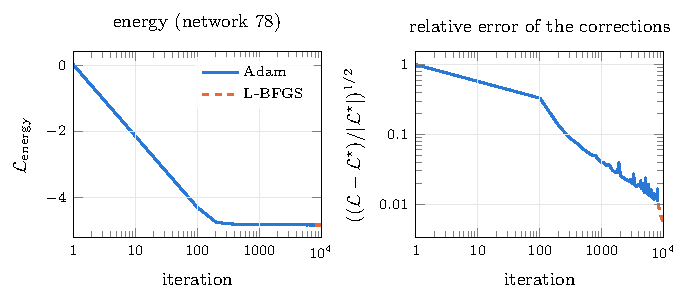
\includegraphics[width=\linewidth,height=0.8\textheight,keepaspectratio]{loss.pdf}
\caption{Training of the network 78: energy loss and relative error of the network corrections in the energy norm (Corollary 3.10) (\texttt{loss})}
\end{figure}
\clearpage
\begin{figure}[htbp]\centering
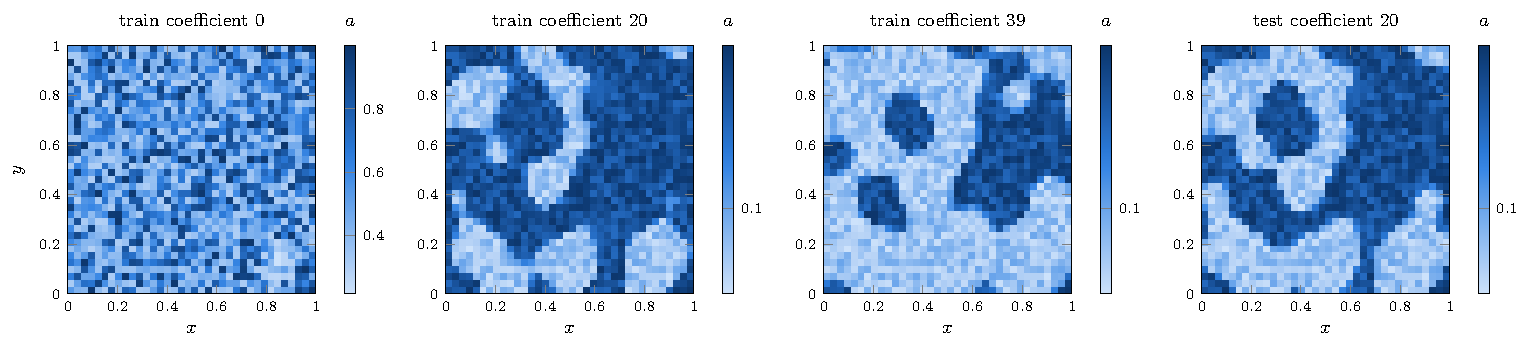
\includegraphics[width=\linewidth,height=0.8\textheight,keepaspectratio]{coefficients.pdf}
\caption{Coefficients of the train set and of the test set (\texttt{coefficients})}
\end{figure}
\clearpage
\begin{figure}[htbp]\centering
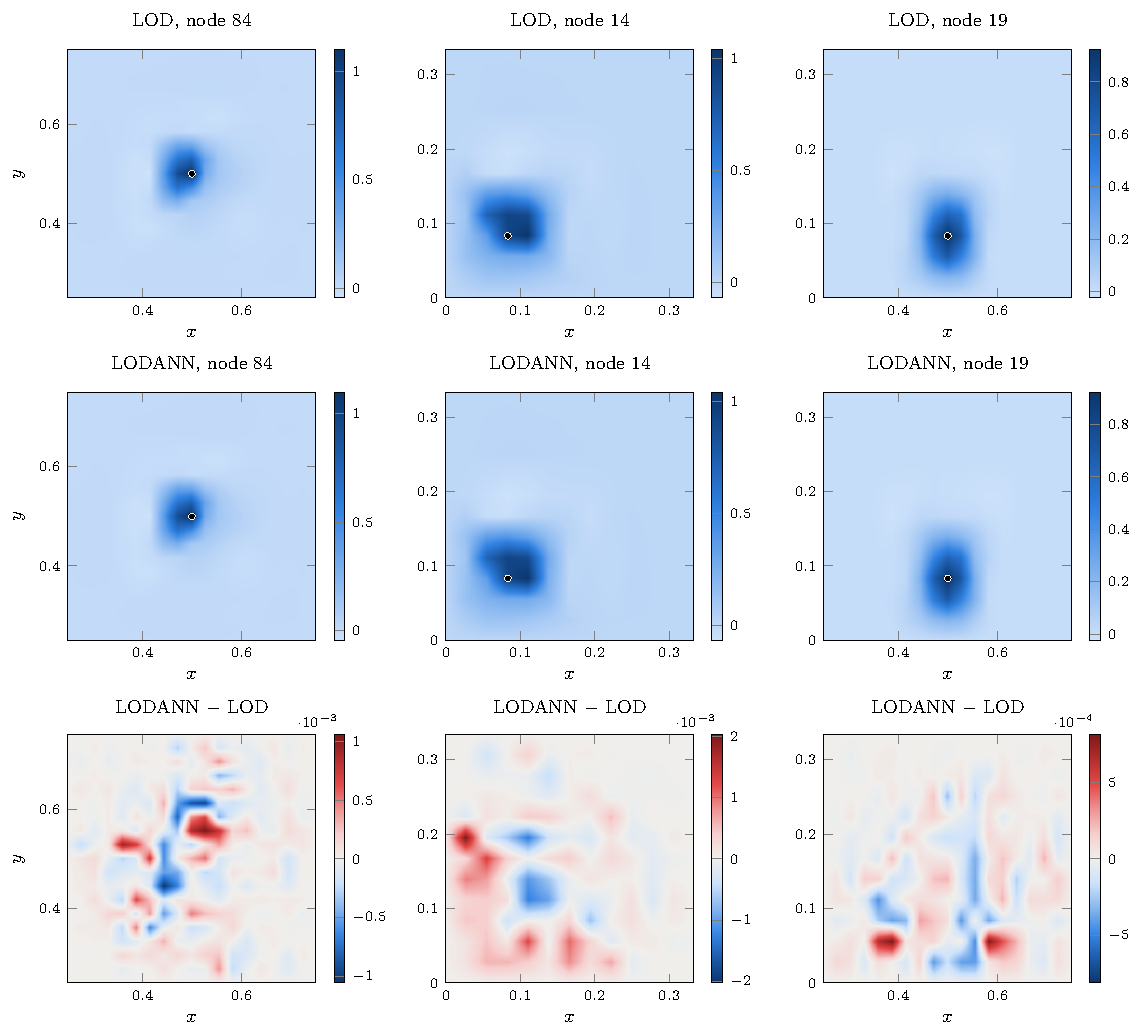
\includegraphics[width=\linewidth,height=0.8\textheight,keepaspectratio]{basis_functions.pdf}
\caption{Corrected basis functions of LOD and DR-LOD and their difference (test coefficient 20) (\texttt{basis\_functions})}
\end{figure}
\clearpage
\begin{figure}[htbp]\centering
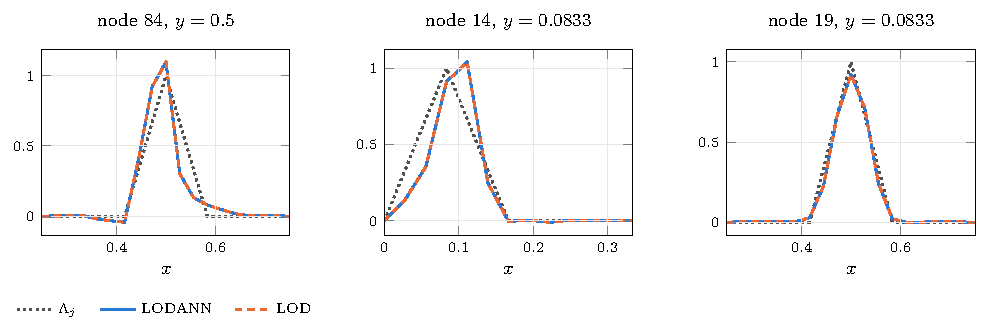
\includegraphics[width=\linewidth,height=0.8\textheight,keepaspectratio]{basis_cross_sections.pdf}
\caption{Cross sections of the basis functions through the node (\texttt{basis\_cross\_sections})}
\end{figure}
\clearpage
\begin{figure}[htbp]\centering
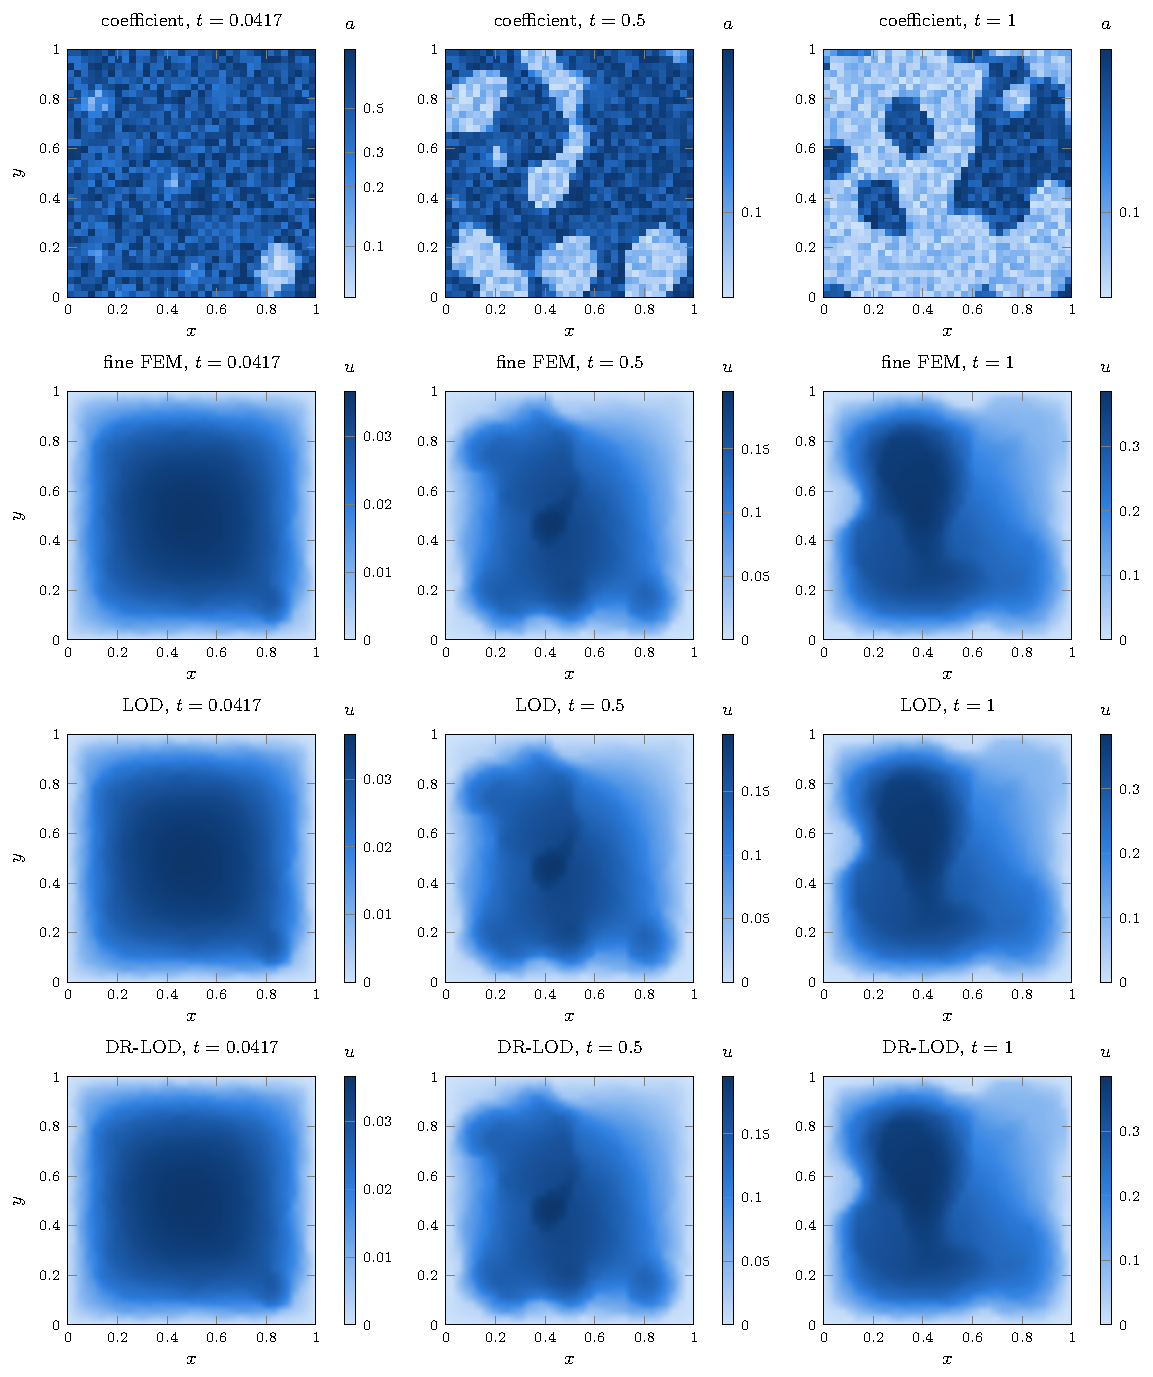
\includegraphics[width=\linewidth,height=0.8\textheight,keepaspectratio]{solutions.pdf}
\caption{Coefficient, fine FEM (reference), LOD and DR-LOD solution (test set) (\texttt{solutions})}
\end{figure}
\clearpage
\begin{figure}[htbp]\centering
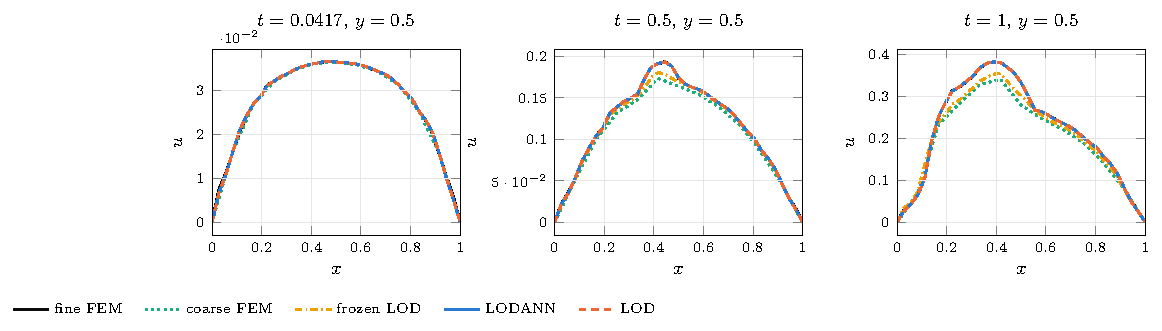
\includegraphics[width=\linewidth,height=0.8\textheight,keepaspectratio]{solution_cross_sections.pdf}
\caption{Cross sections of the solutions of all methods (test set) (\texttt{solution\_cross\_sections})}
\end{figure}
\clearpage
\begin{figure}[htbp]\centering
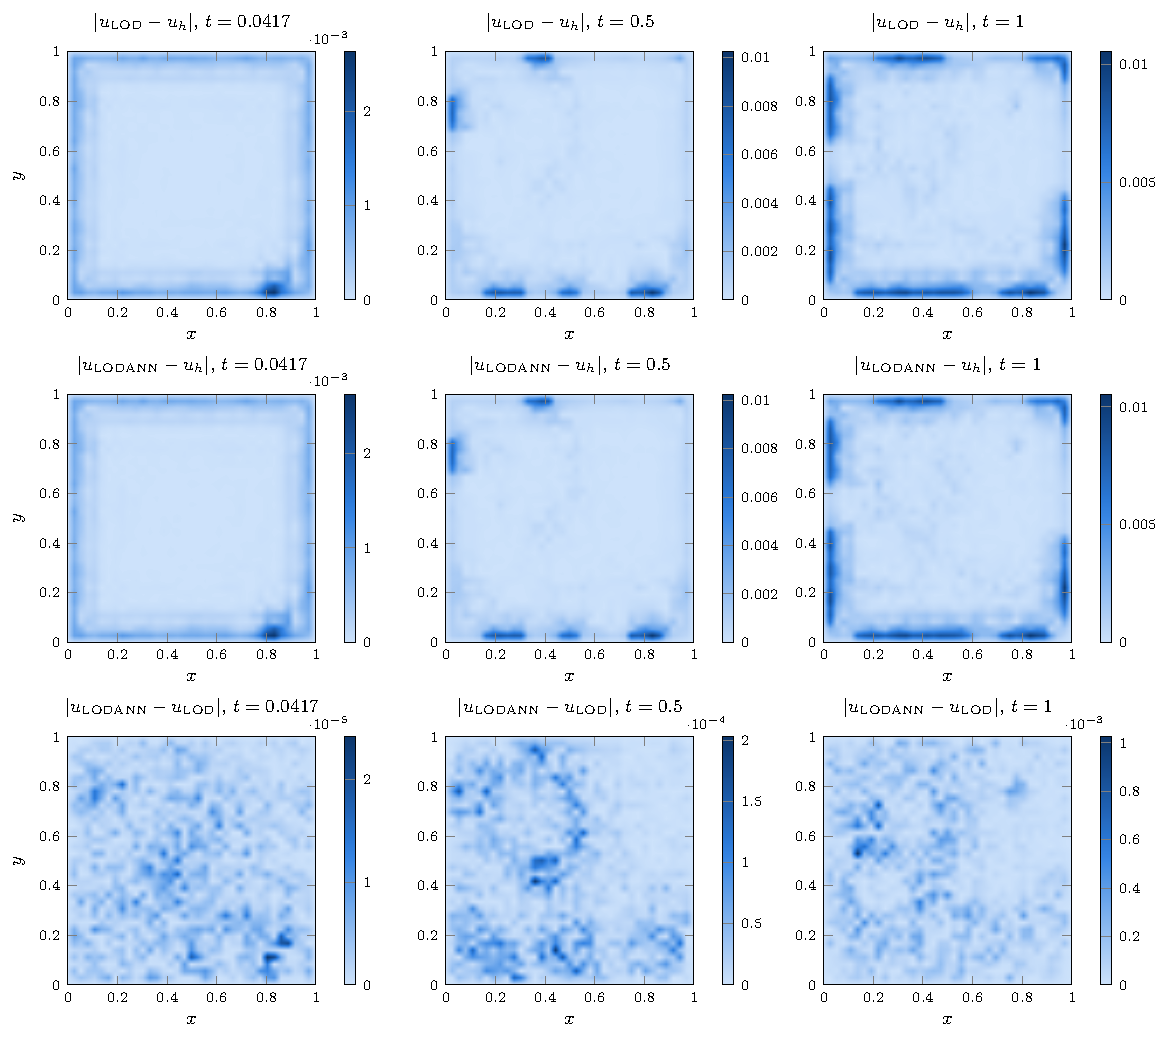
\includegraphics[width=\linewidth,height=0.8\textheight,keepaspectratio]{pointwise_errors.pdf}
\caption{Pointwise errors against the fine FEM solution $u_h$ and between DR-LOD and LOD (test set) (\texttt{pointwise\_errors})}
\end{figure}
\clearpage
\begin{figure}[htbp]\centering
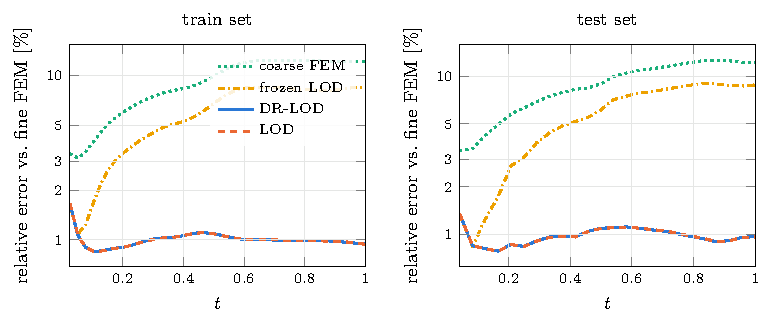
\includegraphics[width=\linewidth,height=0.8\textheight,keepaspectratio]{errors_over_time.pdf}
\caption{Relative error against the fine FEM solution over time (\texttt{errors\_over\_time})}
\end{figure}
\clearpage
\begin{figure}[htbp]\centering
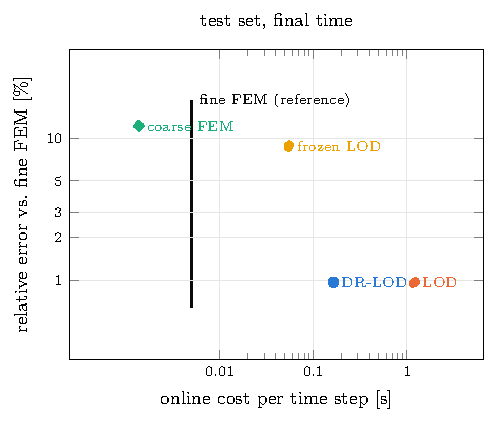
\includegraphics[width=\linewidth,height=0.8\textheight,keepaspectratio]{accuracy_cost.pdf}
\caption{Accuracy against online cost per time step (test set). Fine FEM (reference): 0.00504 s per step; DR-LOD offline training: 5.62 h (recorded). The classical LOD timings refer to the unoptimized implementation in LOD.py. (\texttt{accuracy\_cost})}
\end{figure}
\clearpage
\begin{figure}[htbp]\centering
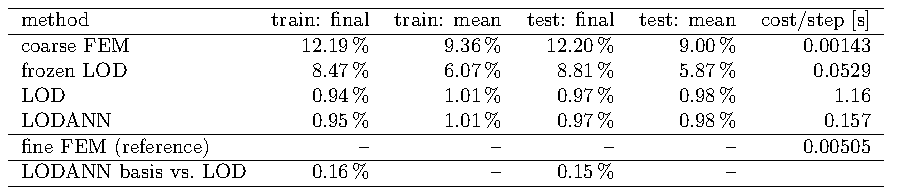
\includegraphics[width=\linewidth,height=0.8\textheight,keepaspectratio]{summary_table.pdf}
\caption{Relative errors against the fine FEM solution (final time and mean over time) and online cost per time step (\texttt{summary\_table})}
\end{figure}
\clearpage
\end{document}
